\documentclass{standalone}
\usepackage{tikz}
\usetikzlibrary{shapes.misc, arrows.meta, positioning, bending, fit}

\begin{document}
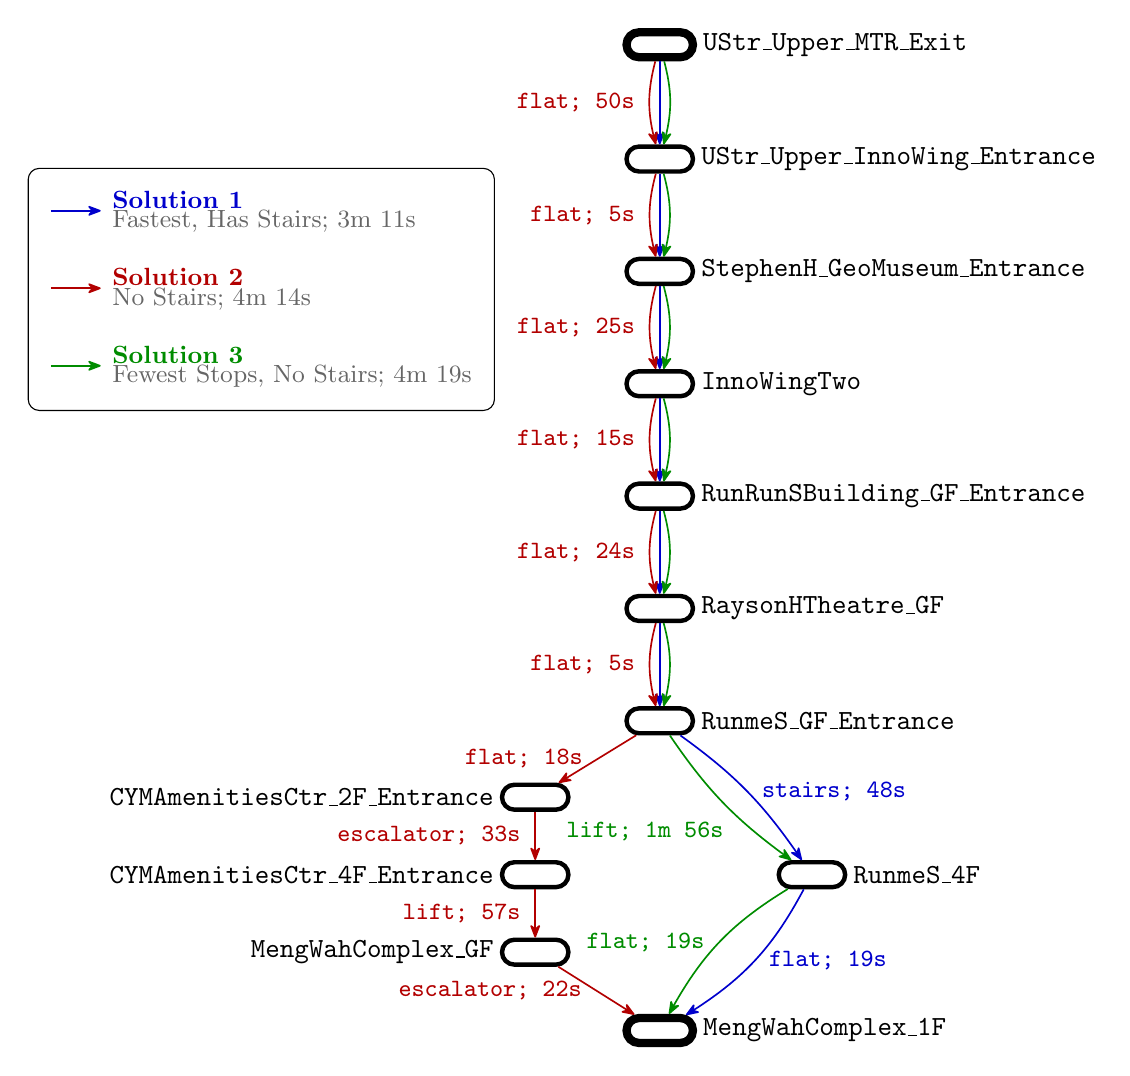
\begin{tikzpicture}[
    %% ── Node styles ──────────────────────────────────────────────────────
    %%
    %% station: small pill/stadium shape used as the "dot" indicator.
    %%   The node body is EMPTY; the monospaced name lives OUTSIDE as a label.
    %%   Edges and positioning are anchored to the pill shape, not the text.
    %%
    %%   Usage:
    %%     \node[station, label={[stlabel]right:NODE\_ID}]               (A) {};
    %%     \node[station-bold, label={[stlabel-bold]right:NODE\_ID}]     (A) {};
    %%
    station/.style={
        draw,
        shape=rounded rectangle,   % from shapes.misc — true semi-circular ends
        rounded rectangle arc length=180,
        minimum height=0.9em,       % height sets the semicircle diameter
        minimum width=2.4em,        % must exceed height to get a flat middle section
        inner xsep=0pt,
        inner ysep=0pt,
        line width=1.6pt,
    },
    %% station-bold + stlabel-bold: use on start/end/waypoint nodes for emphasis.
    station-bold/.style={station, line width=3pt},
    %% stlabel: monospaced name label placed to the right of the station dot.
    %%   Always pass it as the style argument to the label option:
    %%     label={[stlabel]right:NAME}
    stlabel/.style={font=\ttfamily, inner sep=2pt},
    stlabel-bold/.style={stlabel, font=\ttfamily\bfseries},
    %% ── Base directed edge style ───────────────────────────────────────────────
    %%
    %%   All per-solution styles inherit from this.
    %%   For parallel edges use bend left/right:
    %%     \draw[sol1, bend left=20] (A) to node[elabel, above] {label} (B);
    route/.style={
        ->,
        >=Stealth[round],
        semithick,
        % shorten >=4pt,
        % shorten <=4pt,
    },
    %% ── Per-solution edge styles (one colour per solution) ────────────
    %%
    %%   Usage:  \draw[sol1] (A) -- (B);
    %%           \draw[sol2, bend left=20] (A) to node[elabel, above] {text} (B);
    sol1/.style={route, color=blue!80!black},           % Solution 1 — blue
    sol2/.style={route, color=red!70!black},            % Solution 2 — red
    sol3/.style={route, color=green!55!black},          % Solution 3 — green
    sol4/.style={route, color=orange!85!black},         % Solution 4 — orange
    sol5/.style={route, color=violet!80!black},         % Solution 5 — violet
    %% ── Edge label styles ────────────────────────────────────────────────
    %%
    %%   Use the per-solution variant (elabel1–elabel5) so that identical labels
    %%   on parallel edges are still distinguishable by colour.
    %%
    %%   For N parallel edges on the same node pair, spread them symmetrically:
    %%     N=2: bend left=15  /  bend right=15
    %%     N=3: bend left=25  /  straight (no bend)  /  bend right=25
    %%     N=4: bend left=35  /  bend left=12  /  bend right=12  /  bend right=35
    %%
    %%   To additionally separate labels, use xshift on the node option:
    %%     node[elabel3, right, xshift=8pt]
    %%
    %%   Example (2 parallel edges):
    %%     \draw[sol1, bend left=15]  (A) to node[elabel1, left]  {label} (B);
    %%     \draw[sol2, bend right=15] (A) to node[elabel2, right] {label} (B);
    %% ── Legend styles ──────────────────────────────────────────────────────
    %%
    %%   legendtitle: bold coloured solution name — pair with the solution colour.
    %%     e.g. \node[legendtitle, text=blue!80!black] {Solution 1};
    legendtitle/.style={font=\small\bfseries, inner sep=0pt, anchor=west},
    %%   legenddesc: smaller grey text for the lines below the title.
    legenddesc/.style={font=\small, text=black!60, inner sep=0pt, anchor=west},
    elabel/.style ={font=\small\ttfamily, inner sep=5pt},
    elabel1/.style={elabel, text=blue!80!black},
    elabel2/.style={elabel, text=red!70!black},
    elabel3/.style={elabel, text=green!55!black},
    elabel4/.style={elabel, text=orange!85!black},
    elabel5/.style={elabel, text=violet!80!black},
]

%% ── Nodes ────────────────────────────────────────────────────────────────

%% Shared spine (all three solutions)
\node[station-bold, label={[stlabel-bold]right:UStr\_Upper\_MTR\_Exit}]
    (UStr_Upper_MTR_Exit) {};
\node[station, label={[stlabel]right:UStr\_Upper\_InnoWing\_Entrance},
    below=30pt of UStr_Upper_MTR_Exit]
    (UStr_Upper_InnoWing_Entrance) {};
\node[station, label={[stlabel]right:StephenH\_GeoMuseum\_Entrance},
    below=30pt of UStr_Upper_InnoWing_Entrance]
    (StephenH_GeoMuseum_Entrance) {};
\node[station, label={[stlabel]right:InnoWingTwo},
    below=30pt of StephenH_GeoMuseum_Entrance]
    (InnoWingTwo) {};
\node[station, label={[stlabel]right:RunRunSBuilding\_GF\_Entrance},
    below=30pt of InnoWingTwo]
    (RunRunSBuilding_GF_Entrance) {};
\node[station, label={[stlabel]right:RaysonHTheatre\_GF},
    below=30pt of RunRunSBuilding_GF_Entrance]
    (RaysonHTheatre_GF) {};
\node[station, label={[stlabel]right:RunmeS\_GF\_Entrance},
    below=30pt of RaysonHTheatre_GF]
    (RunmeS_GF_Entrance) {};

%% Sol1/Sol3 branch: via RunmeS_4F (right)
\node[station, label={[stlabel]right:RunmeS\_4F},
    below right=45pt and 40pt of RunmeS_GF_Entrance]
    (RunmeS_4F) {};

%% Sol2 branch: via CYMAmenitiesCtr and MengWahComplex_GF (left)
\node[station, label={[stlabel]left:CYMAmenitiesCtr\_2F\_Entrance},
    below left=17pt and 30pt of RunmeS_GF_Entrance]
    (CYMAmenitiesCtr_2F_Entrance) {};
\node[station, label={[stlabel]left:CYMAmenitiesCtr\_4F\_Entrance},
    below left=45pt and 30pt of RunmeS_GF_Entrance]
    (CYMAmenitiesCtr_4F_Entrance) {};
\node[station-bold, label={[stlabel-bold]right:MengWahComplex\_1F},
    below left=45pt and 40pt of RunmeS_4F]
    (MengWahComplex_1F) {};
\node[station, label={[stlabel]left:MengWahComplex\_GF},
    above left=17pt and 30pt of MengWahComplex_1F]
    (MengWahComplex_GF) {};

%% ── Shared spine edges (sol1 straight, sol2 bend right, sol3 bend left) ──

\draw[sol1]               (UStr_Upper_MTR_Exit) -- node[elabel1, right]            {} (UStr_Upper_InnoWing_Entrance);
\draw[sol2, bend right=15](UStr_Upper_MTR_Exit) to node[elabel2, left]             {flat; 50s} (UStr_Upper_InnoWing_Entrance);
\draw[sol3, bend left=15] (UStr_Upper_MTR_Exit) to node[elabel3, right, xshift=20pt]{} (UStr_Upper_InnoWing_Entrance);

\draw[sol1]               (UStr_Upper_InnoWing_Entrance) -- node[elabel1, right]            {} (StephenH_GeoMuseum_Entrance);
\draw[sol2, bend right=15](UStr_Upper_InnoWing_Entrance) to node[elabel2, left]             {flat; 5s} (StephenH_GeoMuseum_Entrance);
\draw[sol3, bend left=15] (UStr_Upper_InnoWing_Entrance) to node[elabel3, right, xshift=20pt]{} (StephenH_GeoMuseum_Entrance);

\draw[sol1]               (StephenH_GeoMuseum_Entrance) -- node[elabel1, right]            {} (InnoWingTwo);
\draw[sol2, bend right=15](StephenH_GeoMuseum_Entrance) to node[elabel2, left]             {flat; 25s} (InnoWingTwo);
\draw[sol3, bend left=15] (StephenH_GeoMuseum_Entrance) to node[elabel3, right, xshift=20pt]{} (InnoWingTwo);

\draw[sol1]               (InnoWingTwo) -- node[elabel1, right]            {} (RunRunSBuilding_GF_Entrance);
\draw[sol2, bend right=15](InnoWingTwo) to node[elabel2, left]             {flat; 15s} (RunRunSBuilding_GF_Entrance);
\draw[sol3, bend left=15] (InnoWingTwo) to node[elabel3, right, xshift=20pt]{} (RunRunSBuilding_GF_Entrance);

\draw[sol1]               (RunRunSBuilding_GF_Entrance) -- node[elabel1, right]            {} (RaysonHTheatre_GF);
\draw[sol2, bend right=15](RunRunSBuilding_GF_Entrance) to node[elabel2, left]             {flat; 24s} (RaysonHTheatre_GF);
\draw[sol3, bend left=15] (RunRunSBuilding_GF_Entrance) to node[elabel3, right, xshift=20pt]{} (RaysonHTheatre_GF);

\draw[sol1]               (RaysonHTheatre_GF) -- node[elabel1, right]            {} (RunmeS_GF_Entrance);
\draw[sol2, bend right=15](RaysonHTheatre_GF) to node[elabel2, left]             {flat; 5s} (RunmeS_GF_Entrance);
\draw[sol3, bend left=15] (RaysonHTheatre_GF) to node[elabel3, right, xshift=20pt]{} (RunmeS_GF_Entrance);

%% ── Diverging edges after RunmeS_GF_Entrance ─────────────────────────────

%% Sol1 → RunmeS_4F via stairs; Sol3 → RunmeS_4F via lift (parallel)
\draw[sol1, bend left=10 ](RunmeS_GF_Entrance) to node[elabel1, right] {stairs; 48s} (RunmeS_4F);
\draw[sol3, bend right=10](RunmeS_GF_Entrance) to  node[elabel3, left, xshift=5pt, yshift=-10pt] {lift; 1m 56s} (RunmeS_4F);

%% Sol1/Sol3 → MengWahComplex_1F (parallel from RunmeS_4F)
\draw[sol1, bend left=15] (RunmeS_4F) to node[elabel1, right]  {flat; 19s} (MengWahComplex_1F);
\draw[sol3, bend right=15](RunmeS_4F) to node[elabel3, left] {flat; 19s} (MengWahComplex_1F);

%% Sol2 → CYMAmenitiesCtr path
\draw[sol2](RunmeS_GF_Entrance)       -- node[elabel2, left] {flat; 18s}      (CYMAmenitiesCtr_2F_Entrance);
\draw[sol2](CYMAmenitiesCtr_2F_Entrance) -- node[elabel2, left] {escalator; 33s} (CYMAmenitiesCtr_4F_Entrance);
\draw[sol2](CYMAmenitiesCtr_4F_Entrance) -- node[elabel2, left] {lift; 57s}      (MengWahComplex_GF);
\draw[sol2](MengWahComplex_GF)        -- node[elabel2, left] {escalator; 22s} (MengWahComplex_1F);

%% ── Legend ───────────────────────────────────────────────────────────────

\begin{scope}[shift={(-220pt, -60pt)}]
    \node[inner sep=0, minimum size=0] (leg-orig) at (0, 0) {};
    \draw[sol1] (0, 0) -- (1.8em, 0);
    \node[legendtitle, text=blue!80!black] (li1-title) at (2.2em,  0.4em) {Solution 1};
    \node[legenddesc]                      (li1-desc)  at (2.2em, -0.4em) {Fastest, Has Stairs; 3m 11s};

    \draw[sol2] (0, -2.8em) -- (1.8em, -2.8em);
    \node[legendtitle, text=red!70!black]  (li2-title) at (2.2em, -2.8em+0.4em) {Solution 2};
    \node[legenddesc]                      (li2-desc)  at (2.2em, -2.8em-0.4em) {No Stairs; 4m 14s};

    \draw[sol3] (0, -5.6em) -- (1.8em, -5.6em);
    \node[legendtitle, text=green!55!black](li3-title) at (2.2em, -5.6em+0.4em) {Solution 3};
    \node[legenddesc]                      (li3-desc)  at (2.2em, -5.6em-0.4em) {Fewest Stops, No Stairs; 4m 19s};

    \node[draw, rounded corners=4pt, inner sep=8pt,
          fit=(leg-orig)(li1-title)(li1-desc)(li2-title)(li2-desc)(li3-title)(li3-desc)
    ] {};
\end{scope}

\end{tikzpicture}
\end{document}
